% ---
% ATENÇÃO: Este arquivo requer o seguinte pacote no preâmbulo:
% \usepackage{longtable}
% ---
% 3 Modelagem do Projeto
% Este arquivo contém a documentação técnica e modelagem do software.
% Conforme as Diretrizes do PPC, deve incluir: levantamento de requisitos,
% diagrama de casos de uso, diagrama de classes, arquitetura do sistema,
% diagrama entidade-relacionamento e interfaces.
% ---
\chapter{MODELAGEM DO PROJETO}
\label{cap:modelagem}

Este capítulo apresenta a documentação técnica e a modelagem do Sistema de Controle de Licença Capacitação, cobrindo aspectos de engenharia de requisitos, design de interface e modelagem de dados, conforme exigido pelas Diretrizes do PPC. O levantamento de requisitos foi realizado com base na legislação federal vigente — Lei nº 8.112/1990, Decreto nº 9.991/2019 e Instrução Normativa SGP-ENAP/SEDGG/ME nº 21/2021 — e nas necessidades identificadas junto ao setor responsável pelo processo na instituição.

\section{Levantamento de Requisitos}

O levantamento de requisitos foi conduzido por meio de análise da legislação vigente e de entrevistas com os responsáveis pelo setor de gestão de pessoas da instituição. O processo atual, realizado manualmente por meio de planilhas eletrônicas, apresenta problemas como conflitos de datas não detectados, ausência de rastreabilidade do fluxo de aprovação e dificuldade no controle do limite legal de servidores afastados simultaneamente. Os requisitos identificados foram organizados em funcionais e não funcionais, conforme apresentado a seguir.

\subsection{Requisitos Funcionais}
Os Requisitos Funcionais (RF) descrevem o que o sistema deve fazer. A Tabela \ref{tab:requisitos_funcionais} apresenta os requisitos funcionais identificados.

\begin{longtable}{|p{1.8cm}|p{1.8cm}|p{6.5cm}|p{4cm}|}
\caption{Lista de Requisitos Funcionais}
\label{tab:requisitos_funcionais} \\

\hline
\textbf{Código} & \textbf{Prioridade} & \textbf{Descrição} & \textbf{Base legal / Justificativa} \\
\hline
\endfirsthead

\hline
\textbf{Código} & \textbf{Prioridade} & \textbf{Descrição} & \textbf{Base legal / Justificativa} \\
\hline
\endhead

\hline
\multicolumn{4}{r}{\small\textit{continua na próxima página}} \\
\endfoot

\hline
\endlastfoot

RF00 & Alta & O sistema deve suportar 4 tipos de afastamento: Licença Capacitação, Participação em Treinamento Regularmente Instituído, Pós-graduação \textit{stricto sensu} no País e Estudo no Exterior. & Art. 18, incisos I a IV, Decreto 9.991/2019 \\ \hline
RF01 & Alta & Cadastrar servidor com dados pessoais, SIAPE e data de ingresso no exercício efetivo. & Necessário para calcular quinquênio (Art. 87, Lei 8.112/1990) \\ \hline
RF02 & Alta & Calcular automaticamente se o servidor completou 5 anos de efetivo exercício. & Decreto 9.991/2019 — requisito de elegibilidade \\ \hline
RF03 & Alta & Controlar saldo de dias conforme o tipo: 90 dias por quinquênio para Licença Capacitação — os demais tipos têm prazos próprios conforme RF12. & Art. 87, Lei 8.112/1990 \\ \hline
RF04 & Alta & Permitir que o servidor registre uma solicitação de licença, com data de início, quantidade de dias e indicação de parcelamento. & Necessidade identificada no processo manual atual \\ \hline
RF05 & Alta & Parcelamento em até 6 períodos com mínimo de 15 dias aplica-se somente ao tipo Licença Capacitação. & Art. 25, §3º, Decreto 9.991/2019 \\ \hline
RF06 & Alta & Observar interstício de 60 dias entre afastamentos, válido entre quaisquer combinações dos 4 tipos. & Art. 27, IN 21/2021 (incisos I a V) \\ \hline
RF07 & Alta & Verificar se o número de servidores simultaneamente afastados não ultrapassa o limite definido pelo órgão, respeitando o teto de 5\%. & Art. 27, Decreto 9.991/2019 \\ \hline
RF08 & Média & Exibir quantos servidores estão de licença no mês atual e projeção para meses futuros. & Problema identificado no processo manual \\ \hline
RF09 & Alta & Alterar status da solicitação entre os estados: pendente, aprovada, negada, em andamento e concluída. & Necessidade de rastreabilidade do processo \\ \hline
RF10 & Média & Registrar histórico de alterações da solicitação, incluindo quem alterou datas ou status e quando. & Resolve o problema de mudanças sem registro no processo manual \\ \hline
RF11 & Média & Gerar relatório ou consulta de dispensa de função gratificada quando a licença for superior a 30 dias. & Art. 18, §1º, Decreto 9.991/2019 \\ \hline
RF12 & Alta & Validar prazo máximo por tipo: mestrado até 24 meses, doutorado até 48 meses, pós-doutorado até 12 meses e estudo no exterior até 4 anos. & Art. 21, Decreto 9.991/2019 \\ \hline
RF13 & Alta & Para afastamentos superiores a 30 dias consecutivos, registrar exoneração ou dispensa de cargo em comissão e suspensão de gratificações vinculadas. & Art. 18, §1º, Decreto 9.991/2019 \\ \hline
RF14 & Média & Para Pós-graduação \textit{stricto sensu}, exigir vínculo com processo seletivo prévio conduzido pela instituição. & Art. 22, Decreto 9.991/2019 \\ \hline
RF15 & Alta & Registrar qual servidor com papel de aprovador decidiu cada solicitação e a data da decisão. & Art. 19, §3º e Art. 28, Decreto 9.991/2019 \\ \hline

\end{longtable}
\legend{Elaborada pelo autor (\imprimirdata).}

\subsection{Requisitos Não Funcionais}
Os Requisitos Não Funcionais (RNF) descrevem restrições e qualidades do sistema:

\begin{longtable}{|p{1.8cm}|p{3cm}|p{9cm}|}
\caption{Lista de Requisitos Não Funcionais}
\label{tab:requisitos_nao_funcionais} \\

\hline
\textbf{Código} & \textbf{Categoria} & \textbf{Descrição} \\
\hline
\endfirsthead

\hline
\textbf{Código} & \textbf{Categoria} & \textbf{Descrição} \\
\hline
\endhead

\hline
\endlastfoot

RNF01 & Integridade de Dados & O sistema deve impedir, via \textit{constraint} de banco de dados — e não apenas por validação na camada de aplicação —, o cadastro de licença com data de fim anterior à data de início. \\ \hline
RNF02 & Desempenho & As consultas de elegibilidade referentes aos requisitos RF02, RF03 e RF07 devem ser resolvidas por meio de \textit{queries} ou \textit{views} no banco de dados, sem recálculo manual na aplicação. \\ \hline
RNF03 & Auditoria & O modelo de dados deve suportar auditoria de alterações — registrando quem alterou o quê e quando — sem duplicar dados entre tabelas. \\ \hline
RNF04 & Usabilidade & A interface do sistema deve ser suficientemente simples para uso por servidores sem familiaridade técnica com sistemas de informação. \\ \hline
RNF05 & Configurabilidade & O percentual máximo de servidores simultaneamente afastados deve ser armazenado como parâmetro configurável do sistema, com valor padrão de 5\%, não podendo ser definido de forma fixa no código da aplicação. \\ \hline

\end{longtable}
\legend{Elaborada pelo autor (\imprimirdata).}

O Quadro \ref{quad:tecnologias} apresenta uma comparação entre as tecnologias avaliadas para o desenvolvimento do sistema.

\begin{table}[htb]
\centering
\caption{Comparação entre tecnologias avaliadas}
\label{quad:tecnologias}
\begin{tabular}{|l|l|l|l|}
\hline
\textbf{Critério} & \textbf{Django} & \textbf{Flask} & \textbf{FastAPI} \\ \hline
Curva de aprendizado & Moderada & Baixa & Baixa \\ \hline
ORM integrado & Sim & Não & Não \\ \hline
Performance & Boa & Boa & Excelente \\ \hline
Documentação & Excelente & Boa & Boa \\ \hline
\end{tabular}
\source{Elaborado pelo autor (\imprimirdata).}
\end{table}


\section{Diagrama de Casos de Uso}

Apresente o Diagrama de Casos de Uso (UML) para ilustrar as interações entre os atores e o sistema. A Figura \ref{fig:caso_uso} apresenta um exemplo.

\begin{figure}[htb]
\centering
\caption{Diagrama de Casos de Uso do Sistema}
\label{fig:caso_uso}
% \includegraphics[width=0.8\textwidth]{figuras/caso_uso.png}
\fbox{\parbox{0.8\textwidth}{\centering \vspace{3cm} [Inserir Imagem do Diagrama de Casos de Uso aqui] \\ Salve a imagem em: \texttt{figuras/caso\_uso.png} \vspace{3cm}}}
\source{Elaborada pelo autor (\imprimirdata).}
\end{figure}

\section{Diagrama de Classes}

Apresente o Diagrama de Classes (UML) que modela a estrutura estática do sistema.

\section{Arquitetura do Sistema}

Descreva a arquitetura adotada (ex: MVC, Cliente-Servidor, Microsserviços). Utilize figuras para ilustrar os componentes e suas interações.

\section{Diagrama Entidade-Relacionamento}

O Modelo Entidade-Relacionamento (MER) do sistema foi construído a partir do levantamento de requisitos legais aplicáveis à concessão de Licença para Capacitação no serviço público federal, contemplando seis entidades principais: \textbf{SERVIDOR}, \textbf{AFASTAMENTO\_VIGENTE}, \textbf{SOLICITACAO}, \textbf{ACAO\_CAPACITACAO}, \textbf{TRAMITACAO} e \textbf{PARCELA}.

O modelo foi elaborado utilizando notação clássica (retângulos para entidades, elipses para atributos, elipses sublinhadas para chaves primárias e losangos para relacionamentos), conforme apresentado na Figura \ref{fig:der_sistema}.

Dentre as regras de negócio incorporadas diretamente na modelagem de dados, destacam-se:

\begin{itemize}
\item o cálculo do saldo de dias de capacitação \textbf{não é armazenado como campo estático}, sendo obtido dinamicamente por meio da soma dos intervalos (\texttt{data\_fim - data\_inicio}) das parcelas com status ``concluída'', evitando inconsistências de dados;
\item a entidade \textbf{TRAMITACAO} reflete o fluxo de aprovação obrigatório definido pelo Art. 33 da IN 21/2021, exigindo três aprovadores: chefia imediata, gestão de pessoas e autoridade máxima;
\item a entidade \textbf{AFASTAMENTO\_VIGENTE} permite a verificação de conflitos entre diferentes tipos de afastamento ativos, impedindo sobreposição de datas.
\end{itemize}

As demais regras de negócio de maior complexidade — como a verificação de elegibilidade por quinquênio, o intervalo mínimo de 60 dias entre parcelas (interstício) e o limite de 5\% de afastamento simultâneo por setor — são validadas na camada de aplicação (\textit{backend}), cabendo ao banco de dados apenas a garantia de restrições estruturais simples, em conformidade com a arquitetura de três camadas adotada no projeto (interface, backend e banco de dados).

\begin{figure}[htb]
\centering
\caption{Diagrama Entidade-Relacionamento do Sistema de Licença Capacitação}
\label{fig:der_sistema}
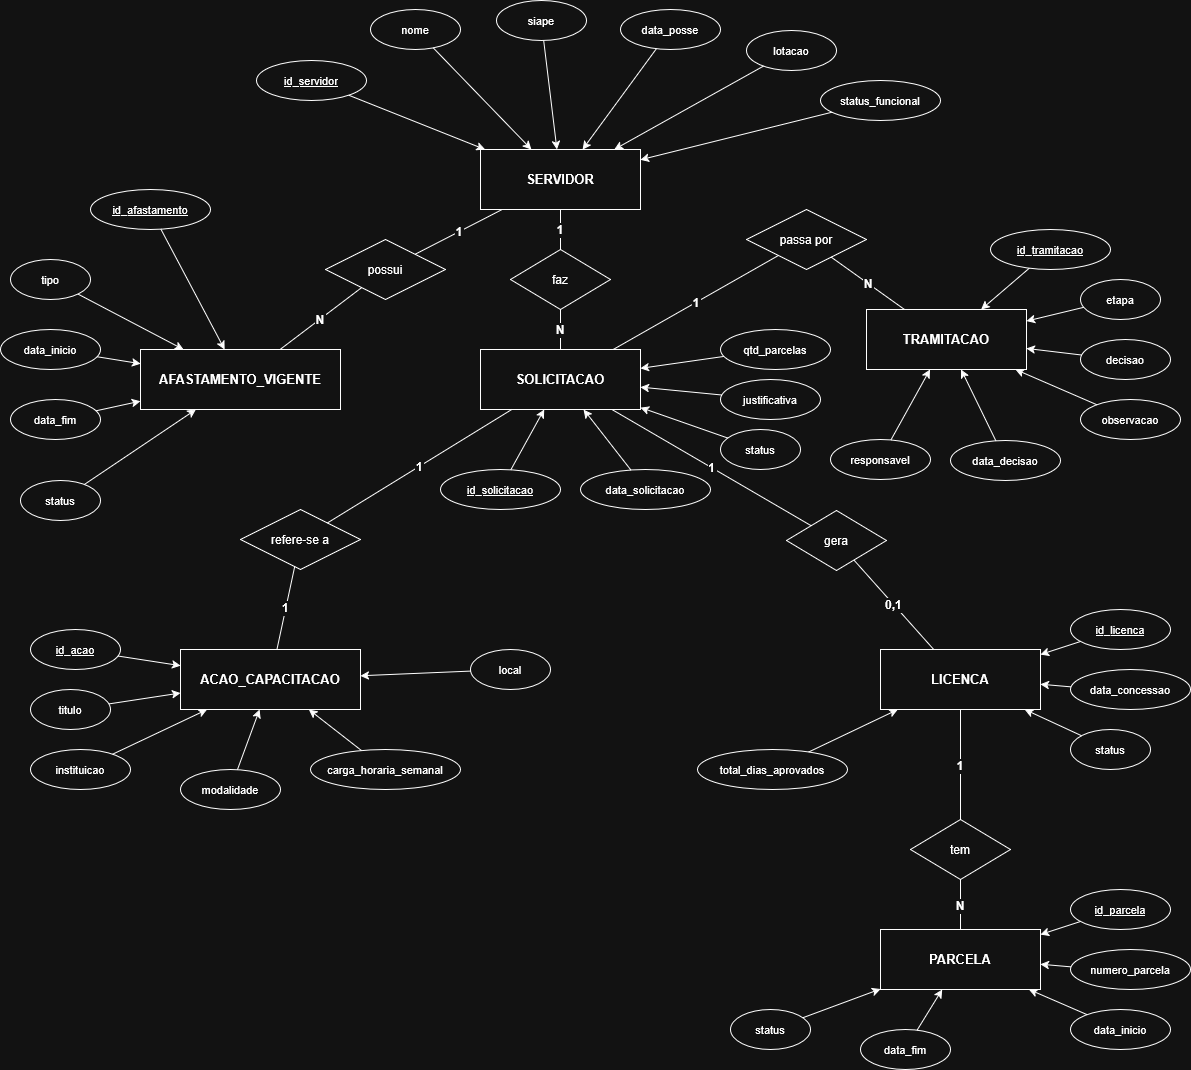
\includegraphics[width=0.95\textwidth]{figuras/der_sistema.png}
\source{Elaborado pelo autor (\imprimirdata).}
\end{figure}

A complexidade algorítmica do módulo de busca foi analisada. A Equação \ref{eq:complexidade} apresenta a complexidade temporal do algoritmo de ordenação utilizado:

\begin{equation}
\label{eq:complexidade}
T(n) = O(n \cdot \log n)
\end{equation}

onde $n$ representa o número de registros a serem ordenados.

\section{Interfaces}

Insira as principais telas do protótipo (\textit{Wireframes} ou \textit{Mockups} de alta fidelidade) desenvolvidas na fase de design. Explique brevemente a funcionalidade de cada tela apresentada.